\documentclass[tikz, border=10pt]{standalone}
\usepackage{tikz}
\usetikzlibrary{shapes.geometric, arrows.meta, positioning, shadows, calc}

% --- UNIVERSITY OF SOUTH CAROLINA MARKETING TOOLBOX COLOR DEFINITIONS ---
% Primary Colors
\definecolor{UofSCGarnet}{RGB}{115, 0, 10}
\definecolor{UofSCBlack}{RGB}{0, 0, 0}
\definecolor{UofSCWhite}{RGB}{255, 255, 255}

% Neutral Colors
\definecolor{UofSC90Black}{RGB}{54, 54, 54}
\definecolor{UofSC70Black}{RGB}{92, 92, 92}
\definecolor{UofSC50Black}{RGB}{162, 162, 162}
\definecolor{UofSC30Black}{RGB}{199, 199, 199}
\definecolor{UofSC10Black}{RGB}{235, 235, 235}
\definecolor{UofSCWarmGrey}{RGB}{103, 97, 86}
\definecolor{UofSCSandstorm}{RGB}{255, 242, 227}

% Accent Colors
\definecolor{UofSCRose}{RGB}{204, 46, 64}
\definecolor{UofSCAtlantic}{RGB}{70, 106, 159}
\definecolor{UofSCCongaree}{RGB}{31, 65, 77}
\definecolor{UofSCHorseshoe}{RGB}{101, 120, 11}
\definecolor{UofSCGrass}{RGB}{206, 211, 24}
\definecolor{UofSCHoneycomb}{RGB}{164, 145, 55}

% Special Use Colors
\definecolor{UofSCDarkGarnet}{RGB}{87, 0, 8}
\definecolor{UofSCAzalea}{RGB}{132, 66, 71}

\begin{document}

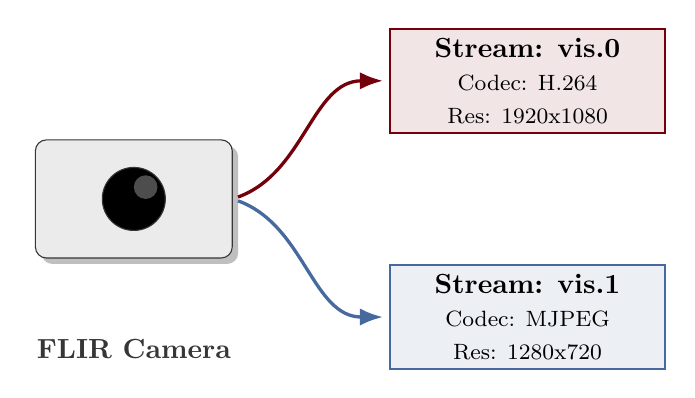
\begin{tikzpicture}[
    >=LaTeX,
    % Define styles for the elements
    camera body/.style={
        rectangle, 
        rounded corners, 
        draw=UofSC90Black,      % Dark Grey outline
        fill=UofSC10Black,      % Light Grey fill
        minimum width=2.5cm, 
        minimum height=1.5cm,
        drop shadow
    },
    camera lens/.style={
        circle, 
        draw=UofSC90Black, 
        fill=UofSCBlack,        % UofSC Black
        inner sep=0pt, 
        minimum size=0.8cm
    },
    stream box/.style={
        rectangle, 
        draw=#1,                % Use passed color for border
        fill=#1!10,             % Use 10% opacity of passed color for fill
        thick, 
        align=center, 
        minimum width=3.5cm, 
        minimum height=1.2cm,
        text=UofSCBlack         % Ensure text is black for readability
    },
    connection line/.style={
        ->, 
        very thick, 
        color=#1, 
        shorten <=2pt, 
        shorten >=2pt
    }
]

    % --- Camera Drawing ---
    % Main body
    \node[camera body] (cam) at (0,0) {};
    % Lens
    \node[camera lens] (lens) at (cam.center) {};
    % Lens reflection/shine
    \fill[white, opacity=0.3] ($(lens.center)+(0.15,0.15)$) circle (0.15cm);
    % Camera label
    \node[below=0.9cm of cam, font=\bfseries, color=UofSC90Black] {FLIR Camera};

    % --- Stream 1: vis.0 (H.264) ---
    % Position: Top Right
    % Using UofSCGarnet (Primary Brand Color) for the primary stream
    \node[stream box=UofSCGarnet] (stream0) at (5, 1.5) {
        \textbf{Stream: vis.0}\\
        \footnotesize Codec: H.264\\
        \footnotesize Res: 1920x1080
    };

    % --- Stream 2: vis.1 (MJPEG) ---
    % Position: Bottom Right
    % Using UofSCAtlantic (Accent Blue) for the secondary stream
    \node[stream box=UofSCAtlantic] (stream1) at (5, -1.5) {
        \textbf{Stream: vis.1}\\
        \footnotesize Codec: MJPEG\\
        \footnotesize Res: 1280x720
    };

    % --- Connections ---
    % Path to Stream 0
    \draw[connection line=UofSCGarnet] (cam.east) to[out=20, in=180] (stream0.west);
    
    % Path to Stream 1
    \draw[connection line=UofSCAtlantic] (cam.east) to[out=-20, in=180] (stream1.west);

\end{tikzpicture}

\end{document}